\documentclass[final]{beamer}
\mode<presentation> {
  \usetheme{UH} 
}
\usepackage{subcaption}
\usepackage{lipsum}
\captionsetup{font=normalsize,labelfont={color=blue,normalsize},compatibility=false}
\usepackage{type1cm}
\usepackage[T1]{fontenc}
\usepackage{amsmath,amsthm, amssymb, latexsym}
\usepackage{multirow}
\usepackage{roboto}
\boldmath
\usepackage[orientation=portrait,size=a0,debug,scale=1.3]{beamerposter}


\bibliographystyle{IEEEtran}
% Reduce bibliography spacing
% https://www.math.cmu.edu/~gautam/sj/blog/20140712-bibtex-spacing.html
% \usepackage{bibspacing}
% \setlength{\bibitemsep}{.2\baselineskip plus .05\baselineskip minus .05\baselineskip}

\title[UH poster]{P52: High-dimensional topological analysis of BOLD sliding window correlations}

\author[Dmitruk]{Emil Dmitruk\textsuperscript{1}, Christoph Metzner\textsuperscript{2}, Volker Steuber\textsuperscript{1} and Shabnam Kadir\textsuperscript{1}
}

% \author[Dmitruk]{Emil Dmitruk\textsuperscript{1}}
% \author[Metzner]{Christoph Metzner\textsuperscript{2}}
% \author[Steuber]{Volker Steuber\textsuperscript{1}}
% \author[Kadir]{Shabnam Kadir\textsuperscript{1}}


\institute[UH]{\textsuperscript{1}University of Hertfordshire, UK; \textsuperscript{2}Technische Universität Berlin, Germany}

\begin{document}
\begin{frame}{} 
  \begin{block}{Introduction}
  \small{
    % \begin{center}
      In recent years, topological insights into neuroscience have brought more understanding about the functional and structural connectivity of the brain \cite{Saggar2018a}\cite{Sizemore2018}. There is evidence that topological properties of brain connectomics are different for schizophrenia subjects and healthy controls \cite{Stolz2018} \cite{Dmitruk2021} but also that the topology can be used to reveal the brain state trajectories \cite{Rieck2020a}. Inspired by those studies we aim to further investigate the brain dynamics and turn our attention to the dynamics of brain pathological states.
      
      
    In this work we aim at establishing the framework for analysis of brain functional dynamics by studying the evolution of its higher-dimensional topological properties.
    We use Midnight Scan Club's~\cite{Gordon2017} fMRI recordings acquired during motor task execution.
    }
    % \end{center}
  \end{block}
  % ===-===-===-===-===-===-===-===-===-===-
      \begin{block}{1. Data and pre-processing.}
      
        \begin{figure}[H]
        \centering
          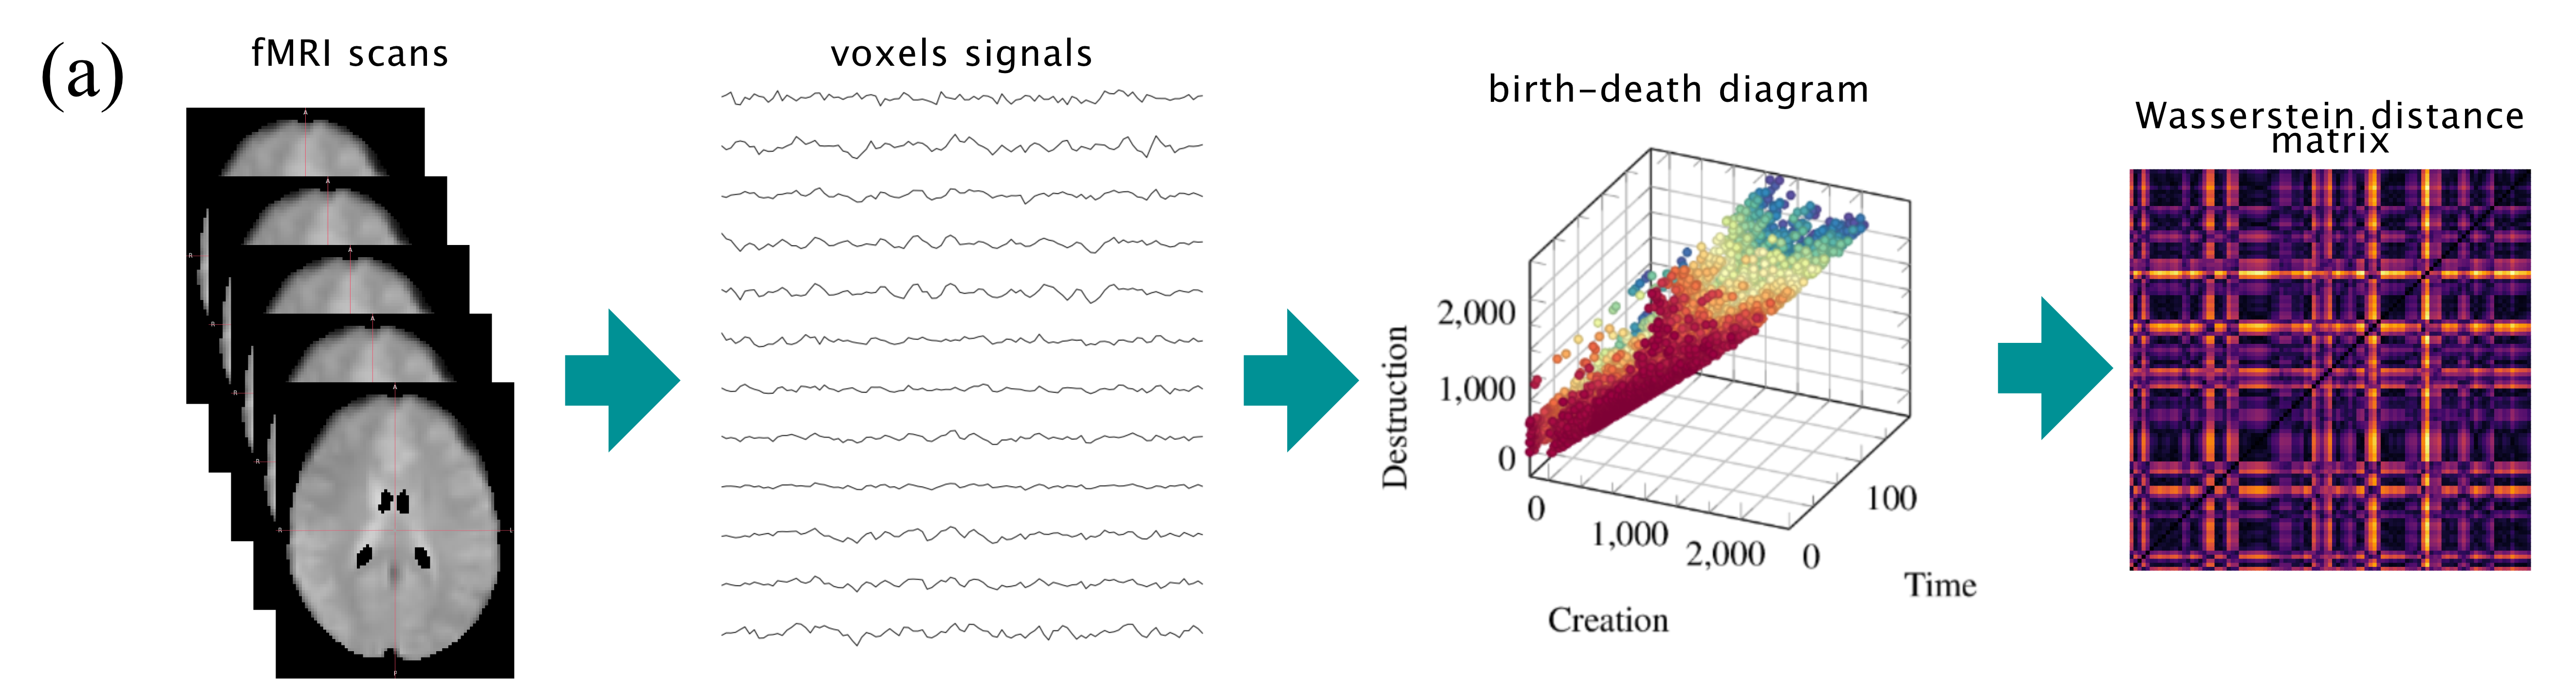
\includegraphics[width=0.7\linewidth]{images/1-preproc.png}
        \label{fig:preproc}
        \end{figure}

        \begin{columns}
        \centering{
        \small{
        
            \begin{column}{0.39\textwidth}
            Preprocessing:
                \begin{itemize}
                \small{
                    \item brain extraction
                    \item spatial smoothing
                    \item ICA-AROMA~\cite{Pruim2015} noise removal
                    \item AAL2~\cite{Rolls2015} motor cortex signal extraction
                    }
                \end{itemize}
          \end{column}
            \begin{column}{0.39\textwidth}
            Topology of time window correlation
                \begin{itemize}
                \small{
                    \item correlation window size: 11 seconds
                    \item sequence of persistence homology characteristic for each of correlation windows
                    \item pairwise Wasserstein distance of persistence characteristics
                    }
                \end{itemize}
          \end{column}
          }
          }
        \end{columns}
      \end{block}
      
  % ===-===-===-===-===-===-===-===-===-===-
  % ===-===-===-===-===-===-===-===-===-===-
%   \begin{columns}

    % ===-===-===-===-===-===-===-===-===-===-
      \begin{block}{2. Topological characteristic of dynamic states}
    \begin{columns}
    \centering{
        \begin{column}{0.5\textwidth}
          
    
          
            \begin{figure}[H]
            \centering
              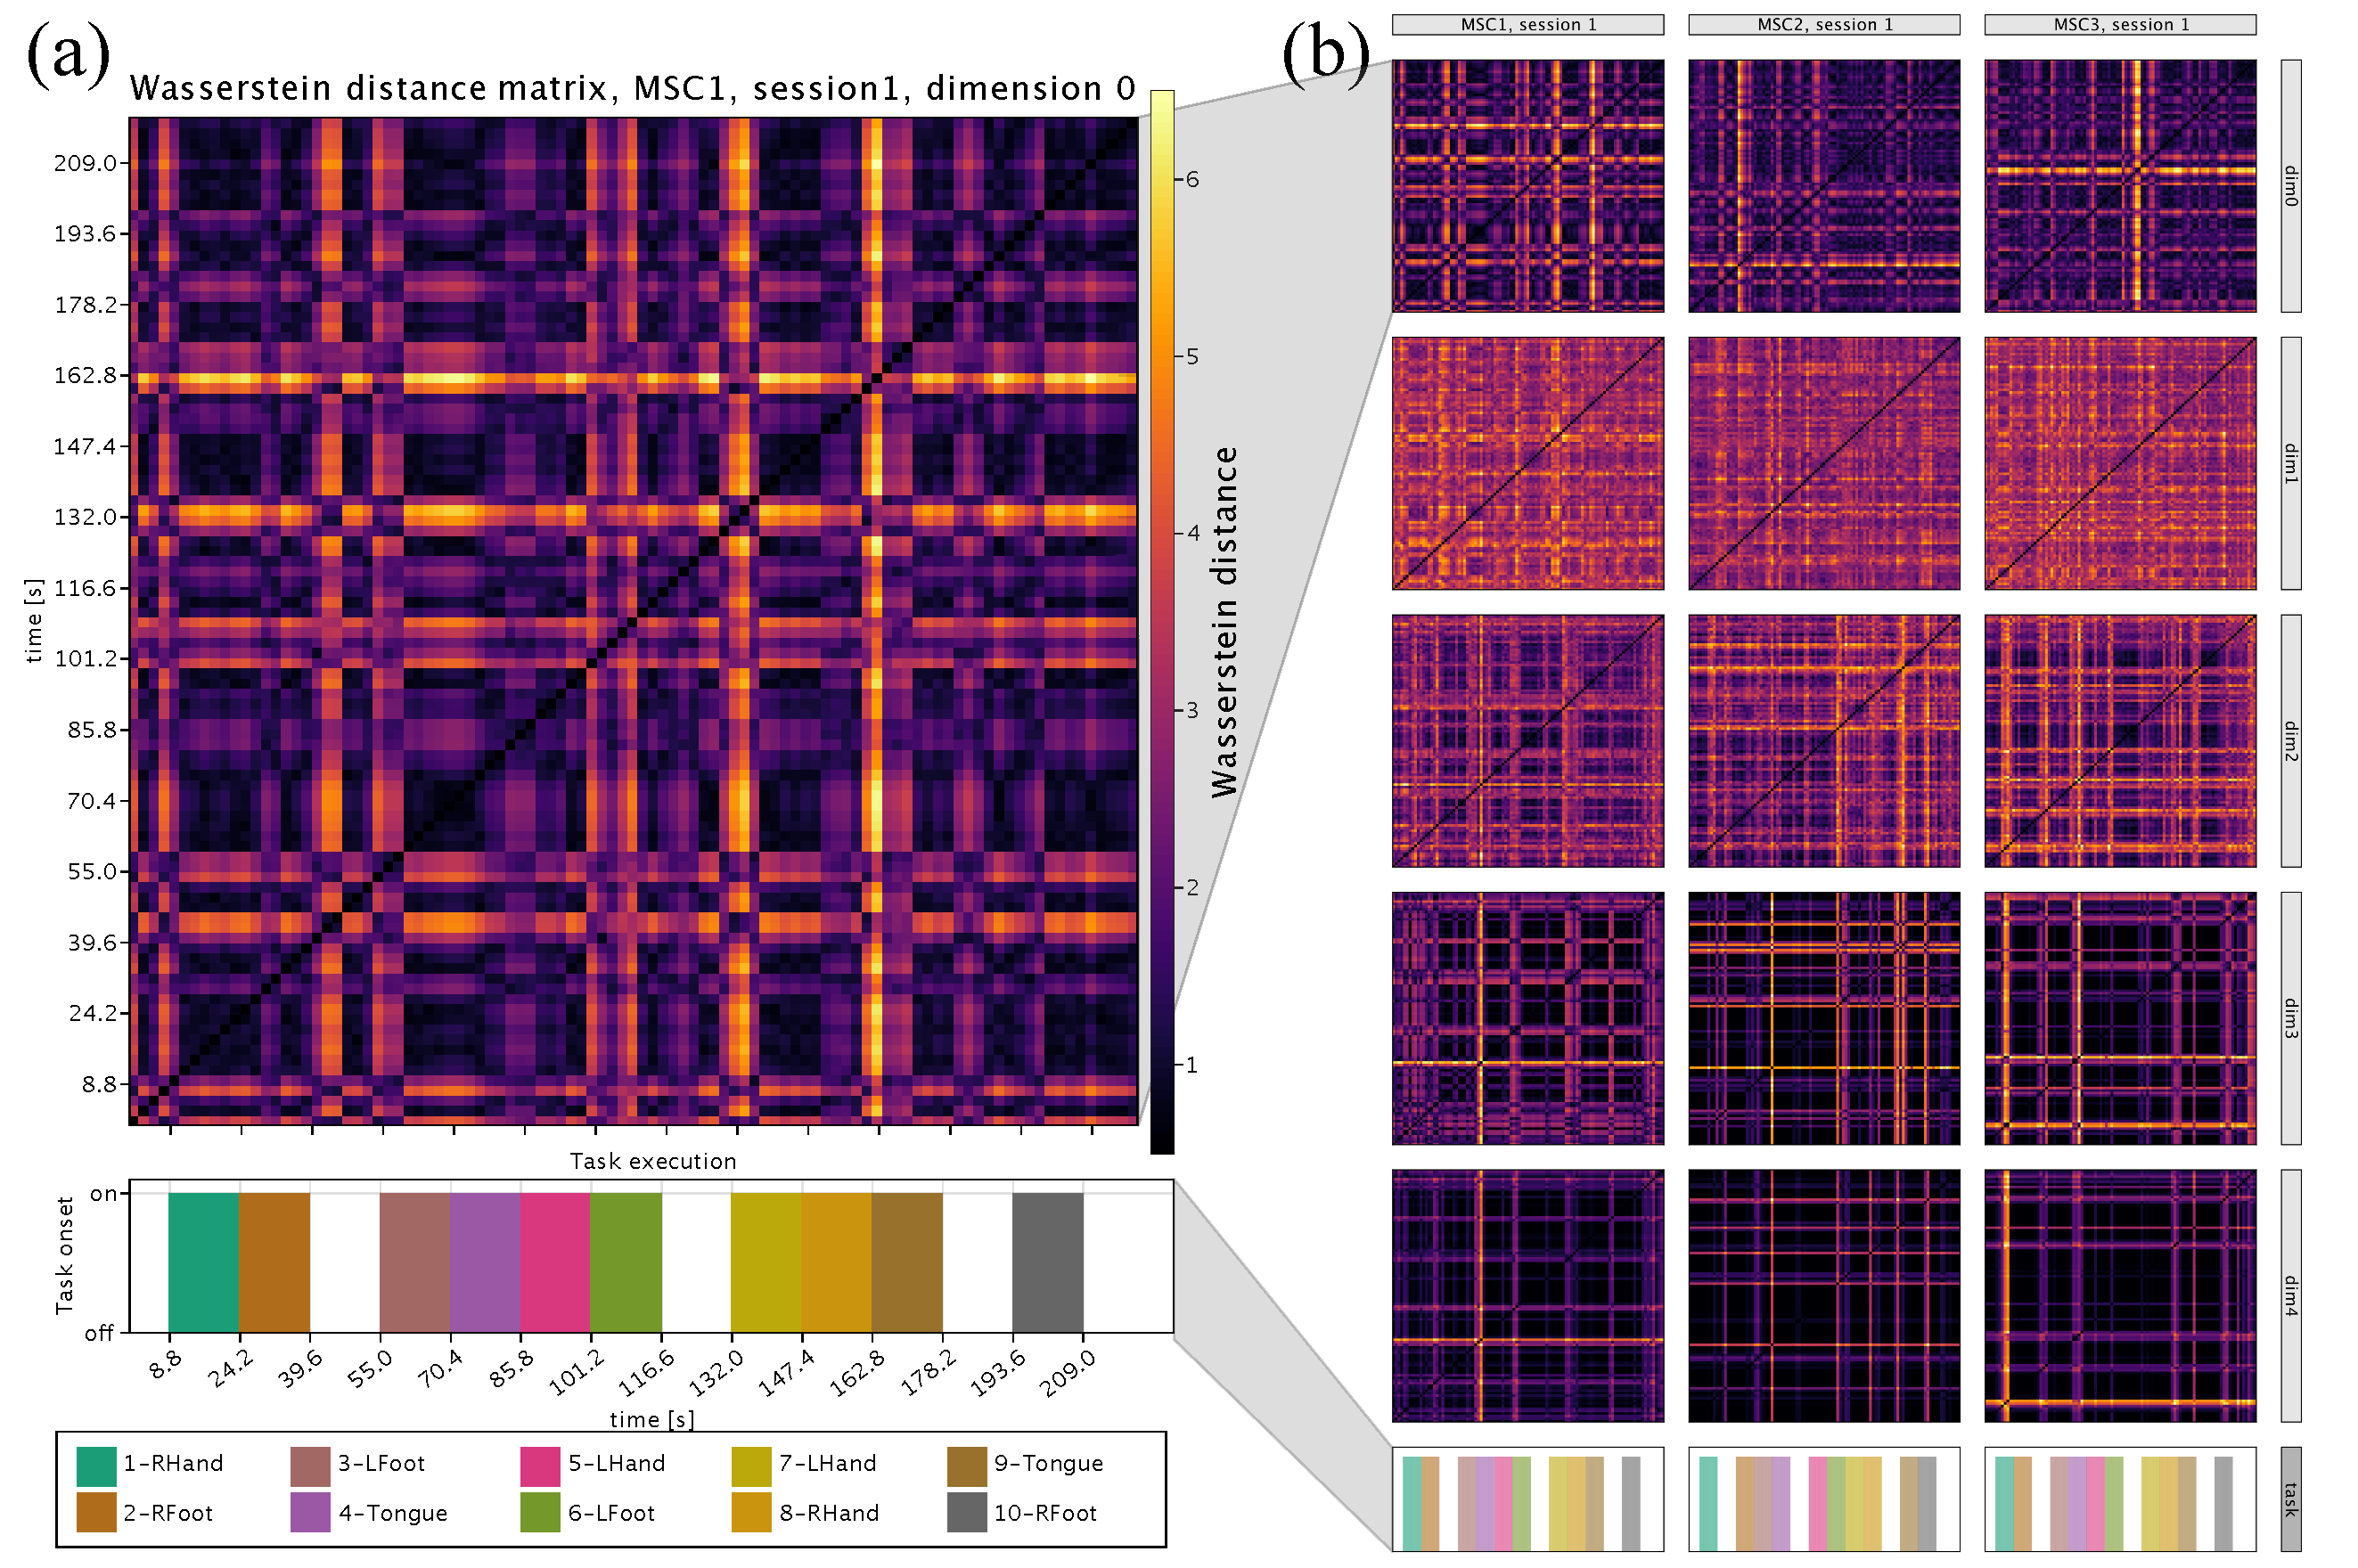
\includegraphics[width=\linewidth]{images/2-wmat.pdf}
            \label{fig:preproc}
            \end{figure}
        \end{column}
        \begin{column}{0.48\textwidth}
        
            \textbf{Results:}
            \begin{itemize}
            \small{
                \item some of the task transitions are correlated in time with the occurrence of higher-ordered topological structures
                \item we hypothesise that those high-dimensional topological structures are related to the brain state transitions
                \item  not all transitions are accompanied by immediate formation of those structures 
                \item the consecutive simplicial complexes are strikingly different
            }
            \end{itemize}
            \;
            
            \;
            
            \textbf{Conclusions:}
            \begin{itemize}
            \small{
                \item first application of high-dimensional topology in the study of dynamics of the brain activity
                \item focus on analysis of the functional connectomics of individuals using just a single recording
                \item better understanding of the differences between individuals’ brain functional connectivities
            }
            \end{itemize}
        \end{column}
            
            % The next step is the investigation of the topological properties of sliding window correlations \cite{Hindriks2016}. 
            % Namely, in each individual single session recording, we compute average signals for each of the brain regions defined in the AAL2~\cite{Rolls2015} atlas. This results in 94 signals of duration 124 samples, for which sliding window correlations is computed (with window size 5 samples). 
            
            % For each correlation window, we derive a clique filtration~\cite{Giusti2015b} and obtain a birth-death diagram, representing brain topological properties- persistence of the cycles~\cite{Zomorodian2005}.  
            } % centering
        \end{columns}
      \end{block}
% ===-===-===-===-===-===-===-===-===-===-
% ===-===-===-===-===-===-===-===-===-===-
    % \end{column}
    
    % \begin{column}{0.3\textwidth}
    % ===-===-===-===-===-===-===-===-===-===-
    %   \begin{block}{3. Topological characteristic.}
    %   \begin{figure}[H]
    %     \centering
    %       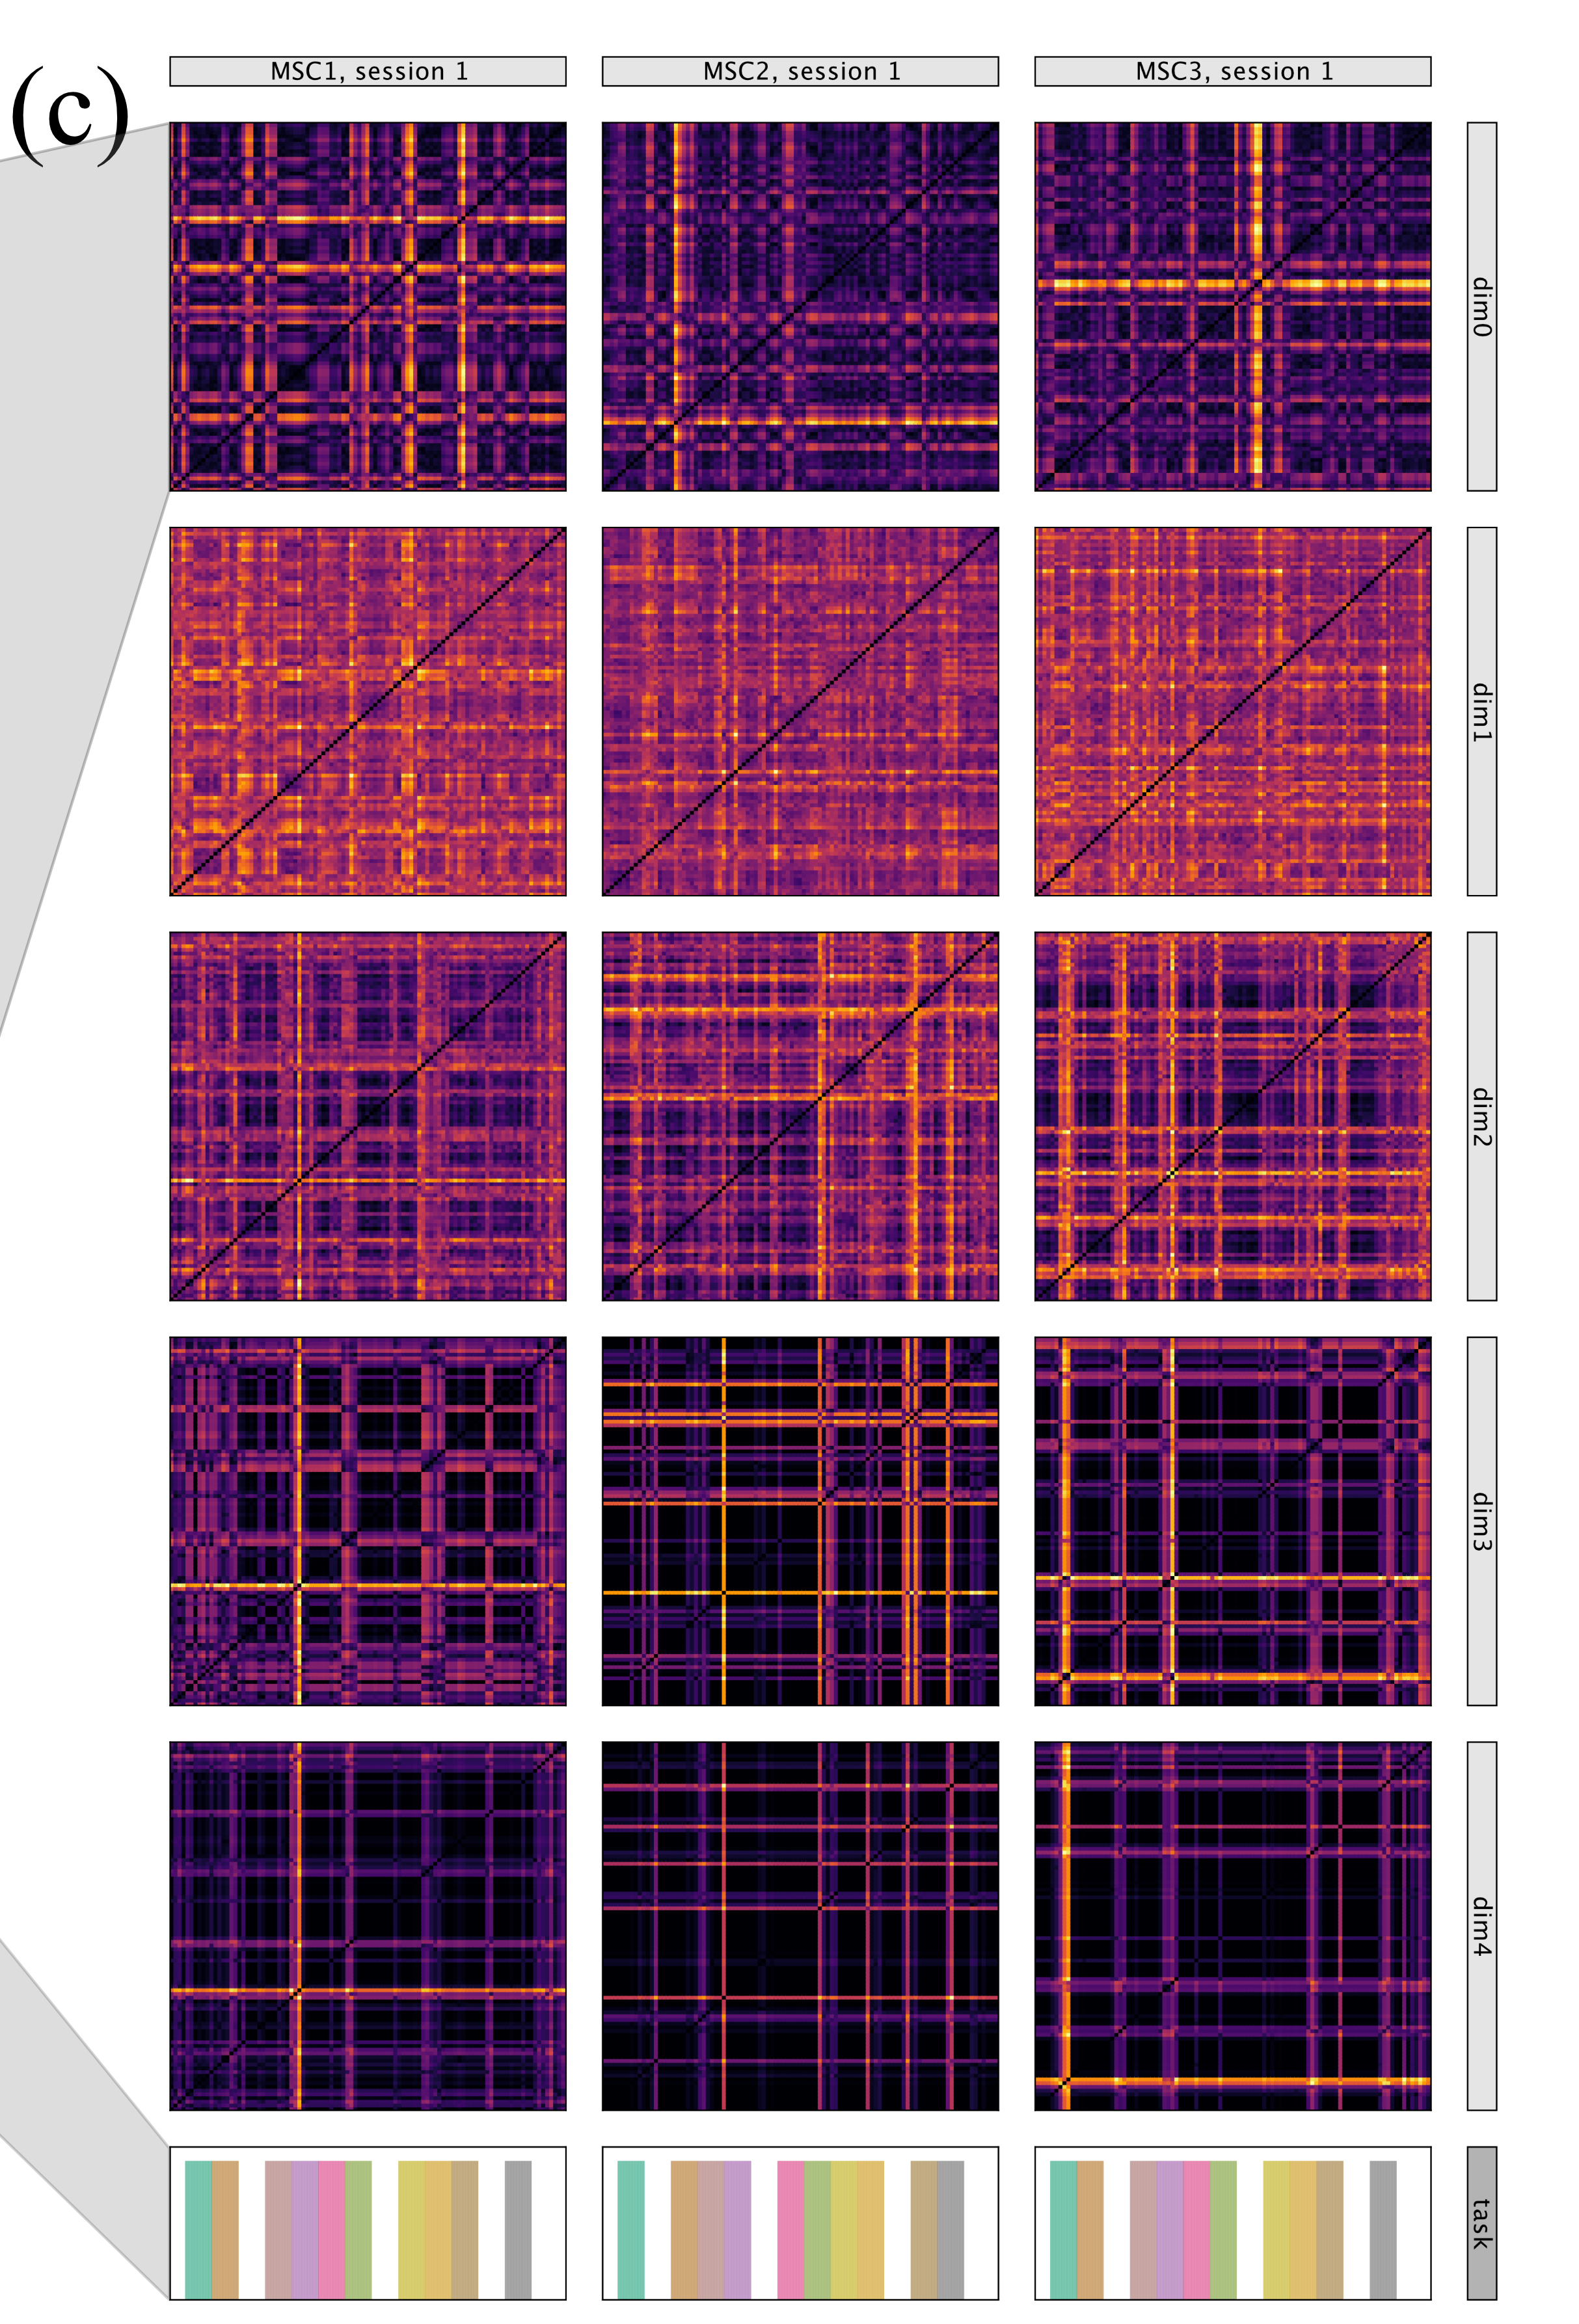
\includegraphics[width=0.7\linewidth]{images/3-results.png}
    %     \label{fig:preproc}
    %     \end{figure}
    %     In the final step, we compute the Wasserstein distance for all pairs of such birth-death diagrams to investigate how the topological properties are evolving through time during task execution.
    %   \end{block}
    %   \end{column}
    %  \begin{column}{0.3\textwidth}
    % ===-===-===-===-===-===-===-===-===-===-  
    %   \begin{block}{4. Results and conclusions}
    %     Some of the results.
    %   \end{block}  
    % ===-===-===-===-===-===-===-===-===-===-  
    \begin{block}{3. Topological characteristic of dynamic states}
    \begin{figure}[H]
            \centering
              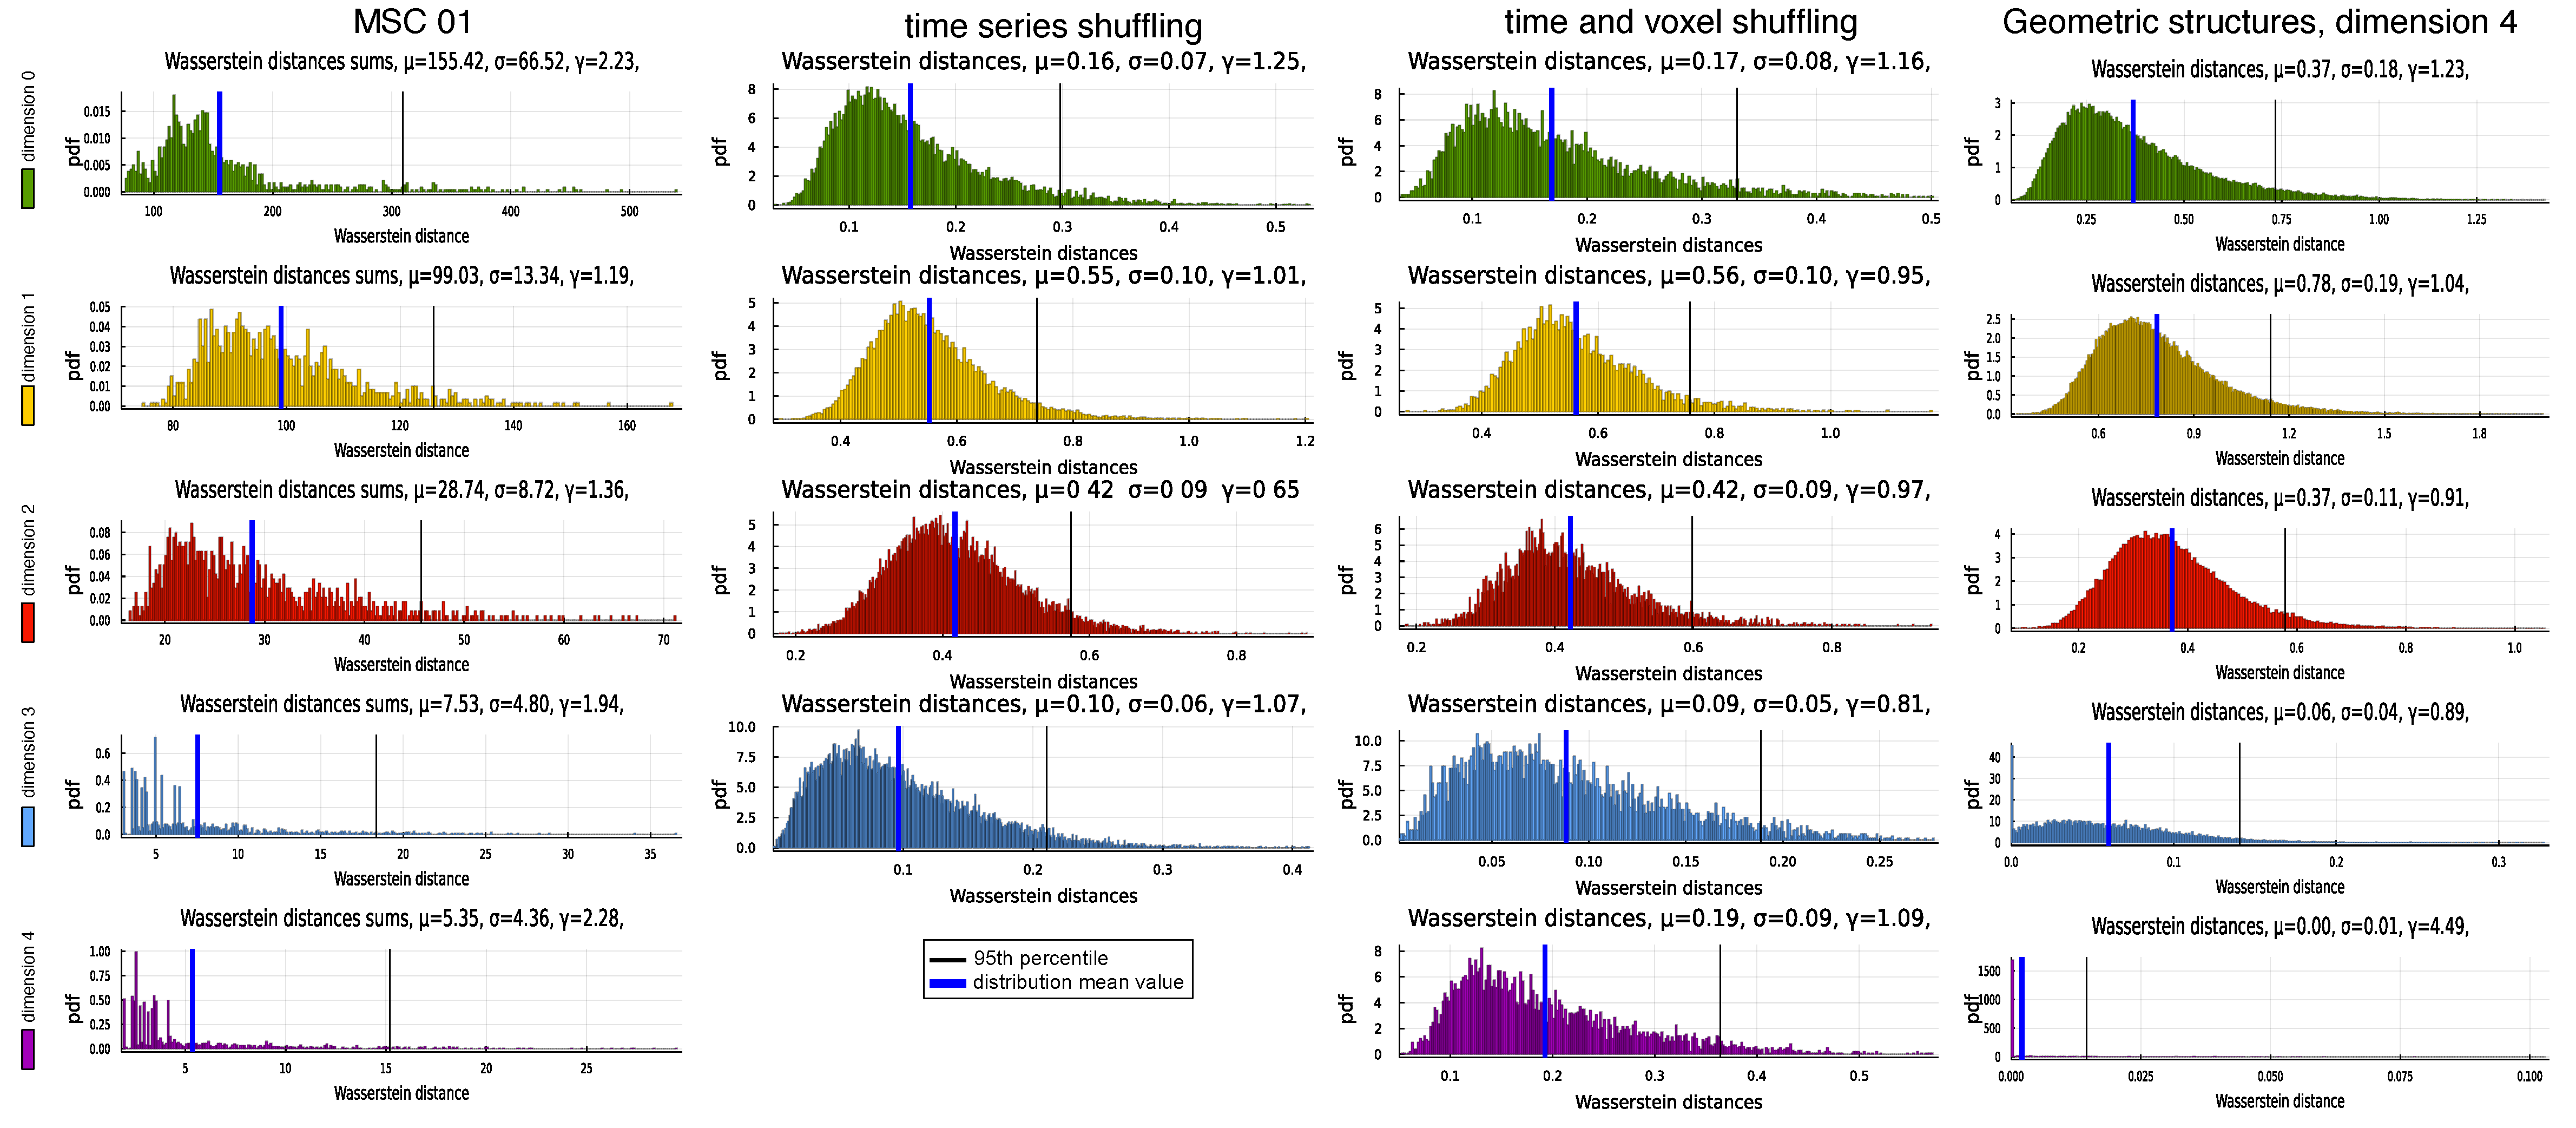
\includegraphics[width=\linewidth]{images/distributions.pdf}
            \label{fig:preproc}
            \end{figure}
    \end{block}
    
    \begin{block}{4. References}
    \tiny{
        \bibliography{biblio2022}
    }
    \end{block}
%     \end{column}
%   \end{columns}
  
  
  
\end{frame}
\end{document}
